% !TeX root = ../main.tex

\begingroup
\raggedbottom
\section{本章例题集}

\begin{workedexample}[由线谱读取奈奎斯特采样频率]
  \label{ex:sampling-nyquist-lines}
  设
  \[
    x(t)=2+\cos(1000\pi t)+\sin(3000\pi t).
  \]
  求 $x$ 的最高频率 $\Omega_M$ 和奈奎斯特采样频率，并画出 $X(\iu\Omega)$ 的实部与虚部。
\end{workedexample}

\begin{solution}
  三项分别使用\cref{eq:ctft-constant-pair,eq:ctft-cosine-pair,eq:ctft-sine-pair}。常数 $2$ 的频谱是
  \[
    2\fourierpair 4\pi\impulse(\Omega).
  \]
  $\cos(1000\pi t)$ 的谱线在 $\pm1000\pi$，权重都是 $\pi$。$\sin(3000\pi t)$ 的变换为
  \[
    \frac{\pi}{\iu}\bigl[\impulse(\Omega-3000\pi)-\impulse(\Omega+3000\pi)\bigr]
    =-\iu\pi\,\impulse(\Omega-3000\pi)
     +\iu\pi\,\impulse(\Omega+3000\pi).
  \]
  \red{实部只含直流和余弦}：零频权重 $4\pi$，$\pm1000\pi$ 的权重各为 $\pi$。\red{虚部只含正弦}：$\Omega=3000\pi$ 处权重的虚部为 $-\pi$，$\Omega=-3000\pi$ 处为 $\pi$。谱线见\cref{fig:ex-sampling-nyquist-lines}。

  非零谱线的最高频率是 $3000\pi$，所以
  \[
    \Omega_M=3000\pi,\qquad 2\Omega_M=6000\pi.
  \]
  奈奎斯特采样频率是 $6000\pi\,\mathrm{rad/s}$。采样定理还要求 $\Omega_s>6000\pi$。换成每秒样数时，$3000\pi t=2\pi\cdot1500\,t$，最高频率为 $1500\,\mathrm{Hz}$，每秒样数要大于 $3000$。不要把 $3000\pi$ 直接读成 $3000\,\mathrm{Hz}$。

  \begin{figure}[H]
    \centering
    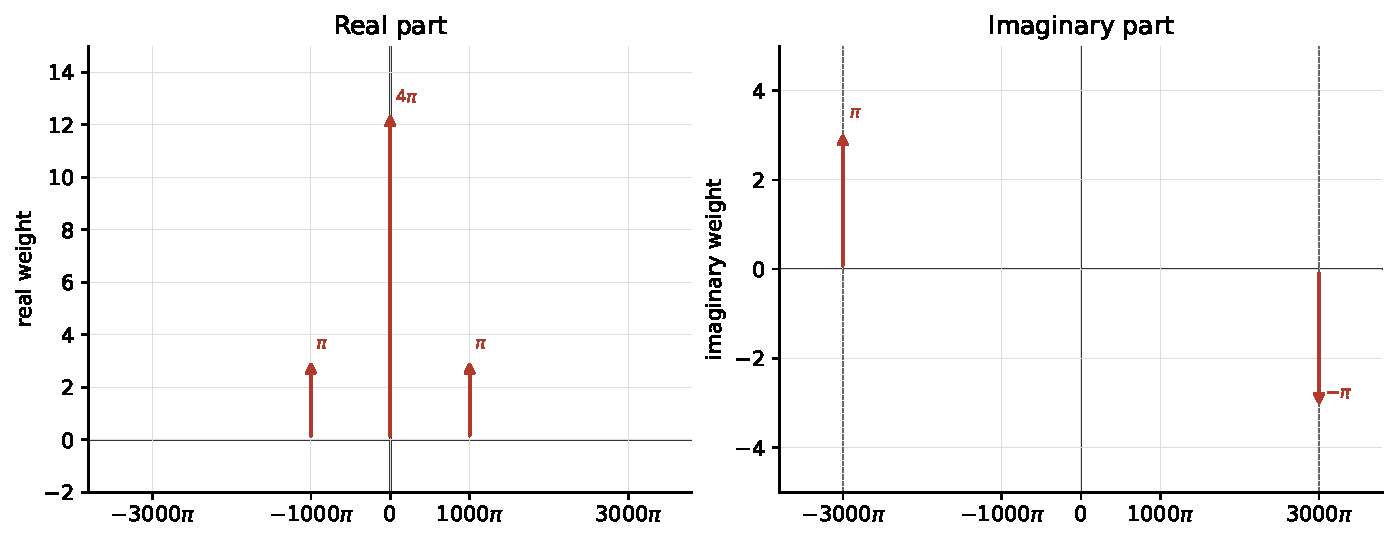
\includegraphics[width=0.92\textwidth]{08-sampling/nyquist-lines.pdf}
    \caption{例题 \ref{ex:sampling-nyquist-lines} 的谱线。左图是实部权重，右图是虚部权重；正弦谱线的复数权重是 $\mp\iu\pi$。}
    \label{fig:ex-sampling-nyquist-lines}
  \end{figure}
\end{solution}

\begin{technique}
  线谱先拆成直流、余弦和正弦。\hl{截止频率取最高一条非零谱线}，权重是实数还是虚数都不改变谱线位置。直流 $A$ 的权重是 $2\pi A$，余弦在正负频率各有一份 $\pi$。奈奎斯特采样频率是 $2\Omega_M$，\blue{实际采样角频率还要严格大于它}。角频率化成赫兹时除以 $2\pi$。
\end{technique}

\begin{workedexample}[平方抽样函数的奈奎斯特采样频率]
  \label{ex:sampling-sinc-square}
  设 $\Omega_c>0$，
  \[
    x(t)=\left(\frac{\sin(\Omega_c t)}{\pi t}\right)^2.
  \]
  求 $X(\iu\Omega)$，并由此确定 $\Omega_M$ 和奈奎斯特采样频率。$t=0$ 处按极限取值。
\end{workedexample}

\begin{solution}
  时域波形见\cref{fig:ex-sampling-sinc-square-time}。图中取 $\Omega_c=1.5$，只用来看主瓣和旁瓣；$\Omega_c$ 变大时主瓣变窄，峰值按 $\Omega_c^2$ 升高。截止频率仍要由下面的频谱支撑决定，\red{不能从波形上估}。

\begin{figure}[H]
  \centering
  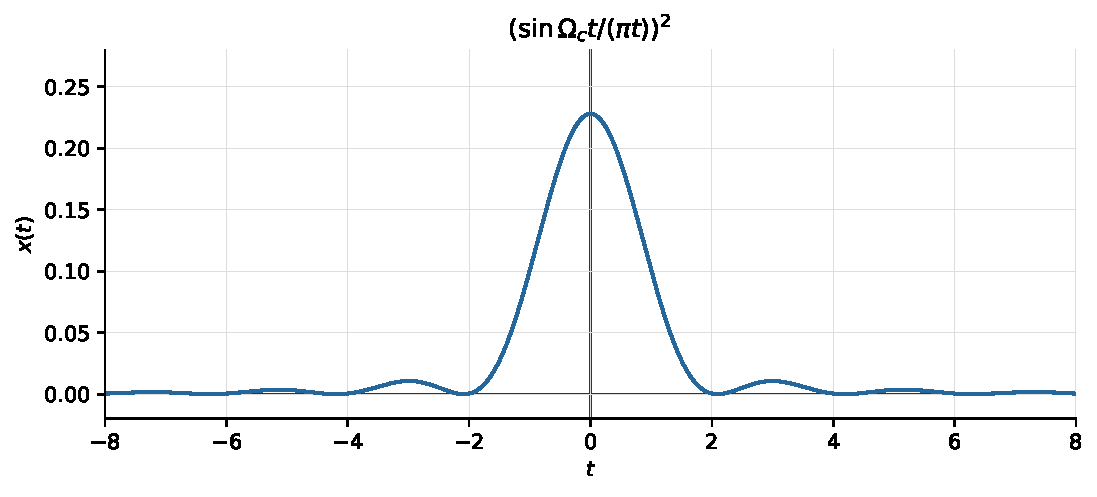
\includegraphics[width=0.72\textwidth]{08-sampling/sinc-square-time.pdf}
    \caption{例题 \ref{ex:sampling-sinc-square} 的时域波形，取 $\Omega_c=1.5$。$t=0$ 处按极限取 $(\Omega_c/\pi)^2$。}
  \label{fig:ex-sampling-sinc-square-time}
\end{figure}

单个因子的矩形频谱是
  \[
    \frac{\sin(\Omega_c t)}{\pi t}
    \fourierpair
    \mathbf{1}_{|\Omega|<\Omega_c}.
  \]
  \red{时域平方对应频域卷积}，并带系数 $1/(2\pi)$：
  \[
    X(\iu\Omega)
    =\frac1{2\pi}
    \bigl(\mathbf{1}_{|\Omega|<\Omega_c}
      \conv\mathbf{1}_{|\Omega|<\Omega_c}\bigr)(\Omega).
  \]
  两个高度为 $1$、宽度为 $2\Omega_c$ 的矩形卷积。$|\Omega|\ge 2\Omega_c$ 时没有重叠；
  $|\Omega|<2\Omega_c$ 时重叠长度是 $2\Omega_c-|\Omega|$，\hl{卷积值就是这个长度}。再除以 $2\pi$，
  \begin{equation}
    X(\iu\Omega)=
    \begin{cases}
      \dfrac{2\Omega_c-|\Omega|}{2\pi},
        &|\Omega|\le 2\Omega_c,\\[0.7em]
      0,&|\Omega|>2\Omega_c.
    \end{cases}
    \label{eq:ex-sampling-sinc-square}
  \end{equation}
  零频高度是 $\Omega_c/\pi$，支撑外缘是 $\pm 2\Omega_c$。因此
  \[
    \Omega_M=2\Omega_c,\qquad 2\Omega_M=4\Omega_c.
  \]
  奈奎斯特采样频率是 $4\Omega_c$，不是平方之前的 $2\Omega_c$。频谱见\cref{fig:ex-sampling-sinc-square}。

  \begin{figure}[H]
    \centering
    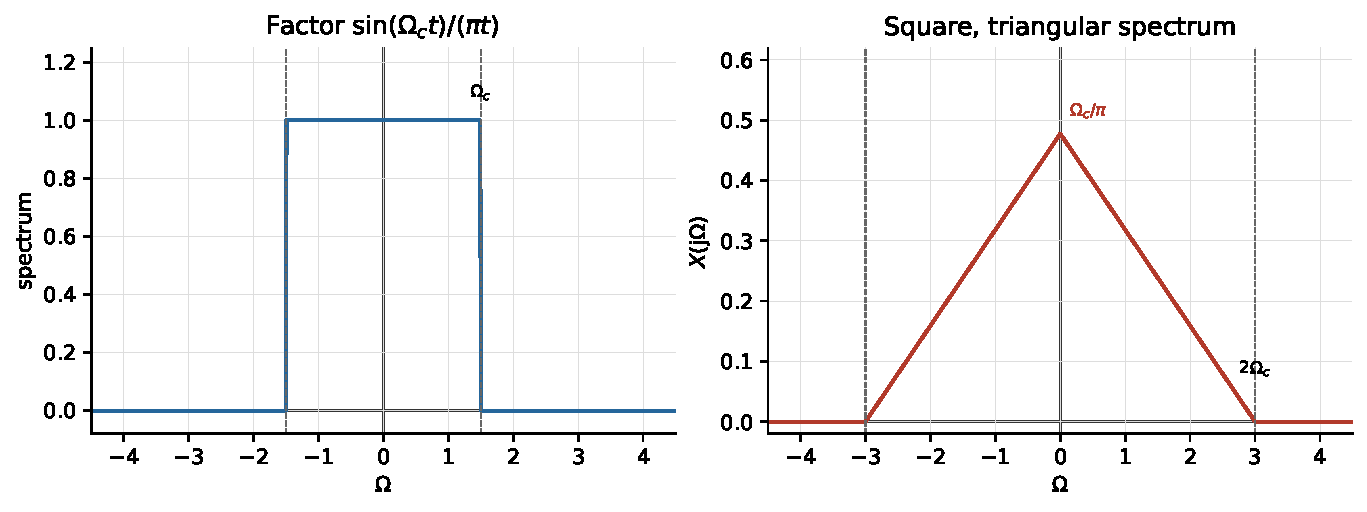
\includegraphics[width=0.92\textwidth]{08-sampling/sinc-square-spectrum.pdf}
    \caption{例题 \ref{ex:sampling-sinc-square} 的频谱。左图是平方前的矩形，右图是卷积后的三角形；三角形在 $\pm 2\Omega_c$ 处降到零，零频高度为 $\Omega_c/\pi$。图中取 $\Omega_c=1.5$，所以零频约 $0.48$。}
    \label{fig:ex-sampling-sinc-square}
  \end{figure}
\end{solution}

\begin{technique}
  \hl{先认清单个因子的矩形边界}，再做频域卷积。\blue{两个单位高度的等宽矩形}卷积后支撑加倍，\red{顶点高度等于原矩形的宽度}，最后还要乘 $1/(2\pi)$。奈奎斯特采样频率按加宽后的外缘计算。若题目写成 $[\sin(\Omega_c t)/t]^2$，每个因子比本题多乘 $\pi$，矩形高度变为 $\pi$，平方后的频谱整体多乘 $\pi^2$。
\end{technique}

\begin{workedexample}[半个样本的延时与周期相位]
  \label{ex:sampling-half-delay}
  已知
  \[
    h[n]=\frac{\sin[\pi(n-1/2)]}{\pi(n-1/2)},\qquad n\in\mathbb Z.
  \]
  求 $H(\e^{\iu\omega})$，画出幅度谱和相位谱。样值见\cref{fig:ex-sampling-half-delay-time}。
\end{workedexample}

\begin{figure}[H]
  \centering
  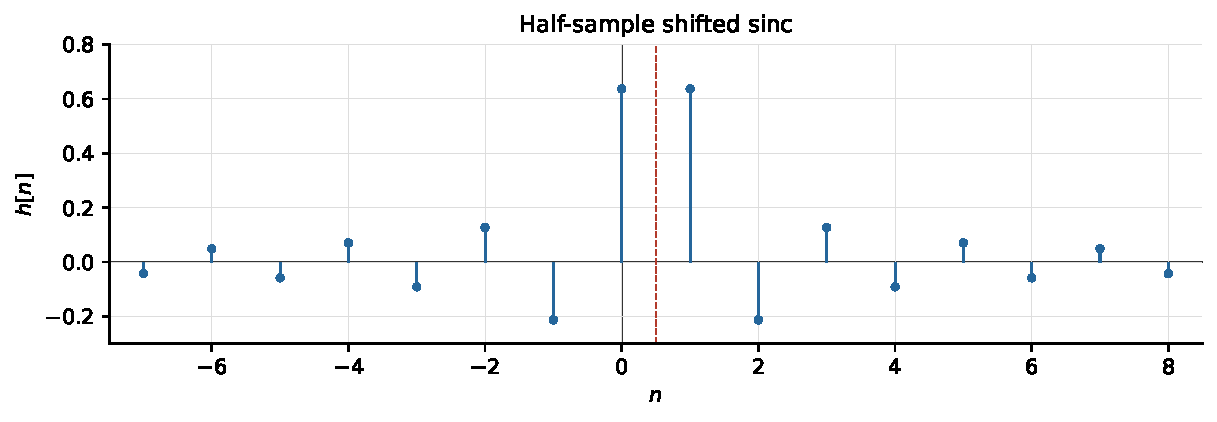
\includegraphics[width=0.77\textwidth]{08-sampling/half-delay-time.pdf}
  \caption{例题 \ref{ex:sampling-half-delay} 的序列。关于 $n=1/2$ 对称，$h[0]=h[1]=2/\pi$，$h[-1]=h[2]=-2/(3\pi)$。}
  \label{fig:ex-sampling-half-delay-time}
\end{figure}

\begin{solution}
  \hl{先构造连续信号}，再取 $T=1$ 的样本：
  \[
    h_c(t)=\sinc(t-1/2),\qquad h[n]=h_c(n).
  \]
  由矩形变换对和时移性质，
  \[
    \sinc(t)\fourierpair\mathbf{1}_{|\Omega|<\pi},
    \qquad
    H_c(\iu\Omega)=
    \begin{cases}
      \e^{-\iu\Omega/2},&|\Omega|<\pi,\\
      0,&|\Omega|>\pi.
    \end{cases}
  \]
  按\cref{eq:sampling-dtft-replicas}，采样把它以 $2\pi$ 为间隔延拓：
  \[
    H(\e^{\iu\omega})=\sum_{k=-\infty}^{\infty}
      H_c\bigl(\iu(\omega-2\pi k)\bigr).
  \]
  在 $-\pi<\omega<\pi$ 内只有中央副本，所以
  \[
    H(\e^{\iu\omega})=\e^{-\iu\omega/2},
    \qquad |H|=1,\qquad \arg H=-\frac{\omega}{2}.
  \]
  其余周期先把频率折回主周期。在
  $(2k-1)\pi<\omega<(2k+1)\pi$ 上，
  \begin{equation}
    H(\e^{\iu\omega})=\e^{-\iu(\omega-2\pi k)/2},
    \qquad \arg H=-\frac{\omega-2\pi k}{2}.
    \label{eq:ex-sampling-half-delay}
  \end{equation}
  例如 $\omega=3\pi/2$ 应折回 $-\pi/2$，相位为 $\pi/4$。直接代入 $-\omega/2$ 会得到 $-3\pi/4$，连复数值都变了。$\e^{-\iu\omega/2}$ 本身是 $4\pi$ 周期，\red{不能把主周期表达式直接用在全实轴}。

  本题的连续带宽恰好为 $\pi$，\blue{不满足前文采样定理的严格不等式}。这里使用有限能量的采样频谱关系：$h[n]$ 平方可和，但不绝对可和，DTFT 按有限能量意义理解。在 $\omega=(2k+1)\pi$ 处，两侧极限分别为 $-\iu$ 和 $\iu$；按傅里叶级数的对称极限，取它们的平均值得 $H=0$。故幅度为 $1$ 是几乎处处成立的结论，接点处幅度为 $0$、相位未定义。\red{改变这些单点的取值不影响逆变换}。

  \begin{figure}[H]
    \centering
    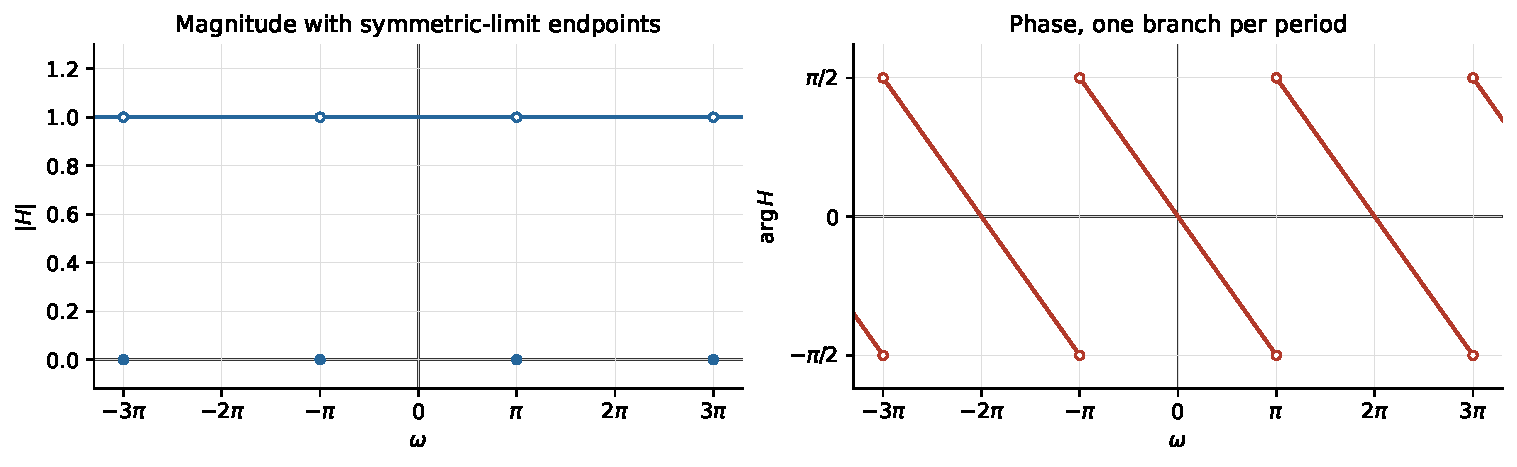
\includegraphics[width=0.93\textwidth]{08-sampling/half-delay-spectrum.pdf}
    \caption{例题 \ref{ex:sampling-half-delay} 的周期幅相谱。奇数倍 $\pi$ 处按对称极限取 $H=0$；相位每周期重新从 $\pi/2$ 降到 $-\pi/2$，跳点不连线。}
    \label{fig:ex-sampling-half-delay-spectrum}
  \end{figure}
\end{solution}

\begin{technique}
  sinc 型序列先找对应的连续信号，用连续变换和时移性质求出一份频谱，再由采样关系作周期延拓。非整数延时尤其要写明主周期：\hl{先折回频率，再代相位}。端点相接时核对复权重及收敛约定，不能只看两份幅度图。
\end{technique}

\begin{workedexample}[冲激采样后通过增益为一的低通]
  \label{ex:sampling-lines-lowpass}
  设 $x(t)=1+\cos t$，采样冲激串为
  \[
    p(t)=\sum_{n=-\infty}^{\infty}\impulse(t-n\pi/3),
    \qquad x_p(t)=x(t)p(t).
  \]
  将 $x_p$ 输入频率响应为
  \[
    H(\iu\Omega)=
    \begin{cases}
      1,&|\Omega|<2,\\
      0,&|\Omega|>2
    \end{cases}
  \]
  的低通系统。求 $X_p(\iu\Omega)$、样本序列 $x[n]=x(n\pi/3)$ 的 DTFT，以及输出 $y(t)$。
\end{workedexample}

\begin{figure}[H]
  \centering
  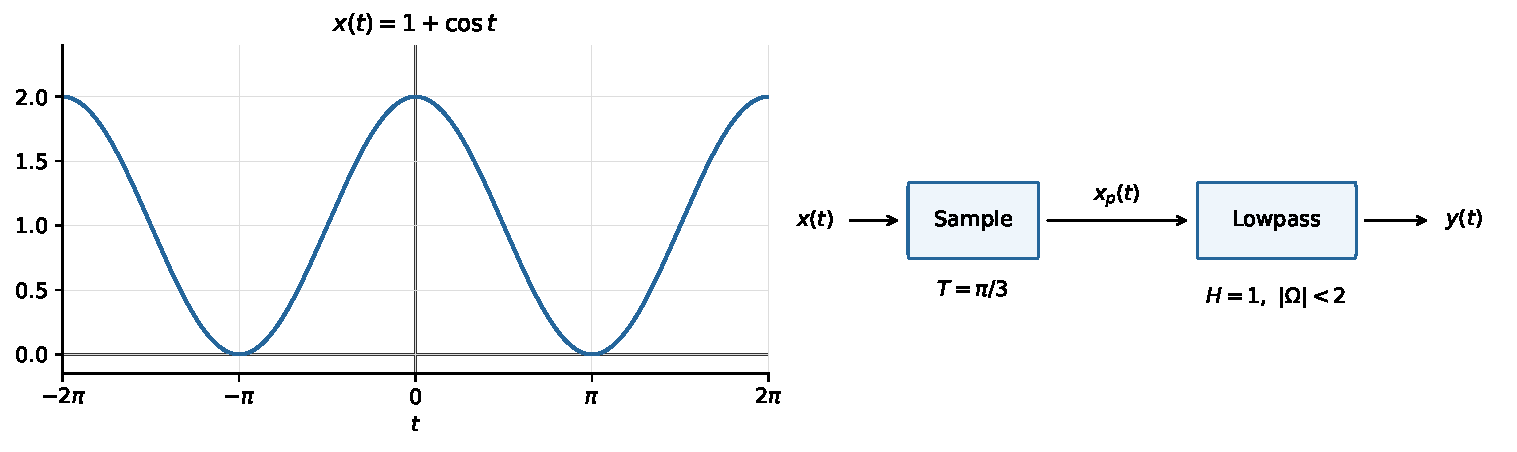
\includegraphics[width=0.92\textwidth]{08-sampling/lines-lowpass-question.pdf}
  \caption{例题 \ref{ex:sampling-lines-lowpass} 的输入与处理路线。采样周期为 $\pi/3$，低通通带高度为 $1$、截止为 $2$。}
  \label{fig:ex-sampling-lines-lowpass-question}
\end{figure}

\begin{solution}
  先求连续频谱：
  \[
    X(\iu\Omega)=2\pi\impulse(\Omega)
       +\pi\bigl[\impulse(\Omega-1)+\impulse(\Omega+1)\bigr].
  \]
  本题 $T=\pi/3$，$\Omega_s=2\pi/T=6$。采样频谱是间隔为 $6$ 的副本，每份权重乘 $1/T=3/\pi$：
  \begin{align*}
    X_p(\iu\Omega)
    &=\frac3\pi\sum_k X\bigl(\iu(\Omega-6k)\bigr)\\
    &=\sum_k\left\{6\impulse(\Omega-6k)
       +3\impulse(\Omega-6k-1)
       +3\impulse(\Omega-6k+1)\right\}.
  \end{align*}
  每组谱线的位置是 $6k-1,6k,6k+1$，权重依次为 $3,6,3$。

  样本序列为 $x[n]=1+\cos(n\pi/3)$，周期是 $6$。一个周期按下标列出：
  \[
    \begin{array}{c|rrrrrr}
      n&0&1&2&3&4&5\\ \hline
      x[n]&2&3/2&1/2&0&1/2&3/2
    \end{array}
  \]
  用 $X(\e^{\iu\omega})=X_p(\iu\omega/T)$ 换轴时，\hl{还要变换冲激权重}：
  \[
    \impulse(\omega/T-a)=T\impulse(\omega-aT).
  \]
  因而 $6T=2\pi$，$3T=\pi$，得到
  \begin{align*}
    X(\e^{\iu\omega})=\sum_k\bigl\{&
      2\pi\impulse(\omega-2\pi k)\\
      &+\pi\impulse(\omega-2\pi k-\pi/3)
       +\pi\impulse(\omega-2\pi k+\pi/3)\bigr\}.
  \end{align*}
  频率位置从 $0,\pm1$ 变成 $0,\pm\pi/3$，\red{权重也相应改变}，不能把 $6,3,3$ 原样搬到离散频率轴上。

  低通只保留中央的 $0,\pm1$ 三条谱线：
  \[
    Y(\iu\Omega)=X_p(\iu\Omega)H(\iu\Omega)
      =6\impulse(\Omega)
       +3\bigl[\impulse(\Omega-1)+\impulse(\Omega+1)\bigr].
  \]
  反演时每条谱线的权重除以 $2\pi$，
  \[
    y(t)=\frac6{2\pi}
       +\frac3{2\pi}(\e^{\iu t}+\e^{-\iu t})
       =\frac3\pi(1+\cos t)=\frac1T x(t).
  \]
  输入满足采样定理，但本题低通的通带增益为 $1$。若要恢复 $x(t)$，该增益应取 $T=\pi/3$。

  \begin{figure}[H]
    \centering
    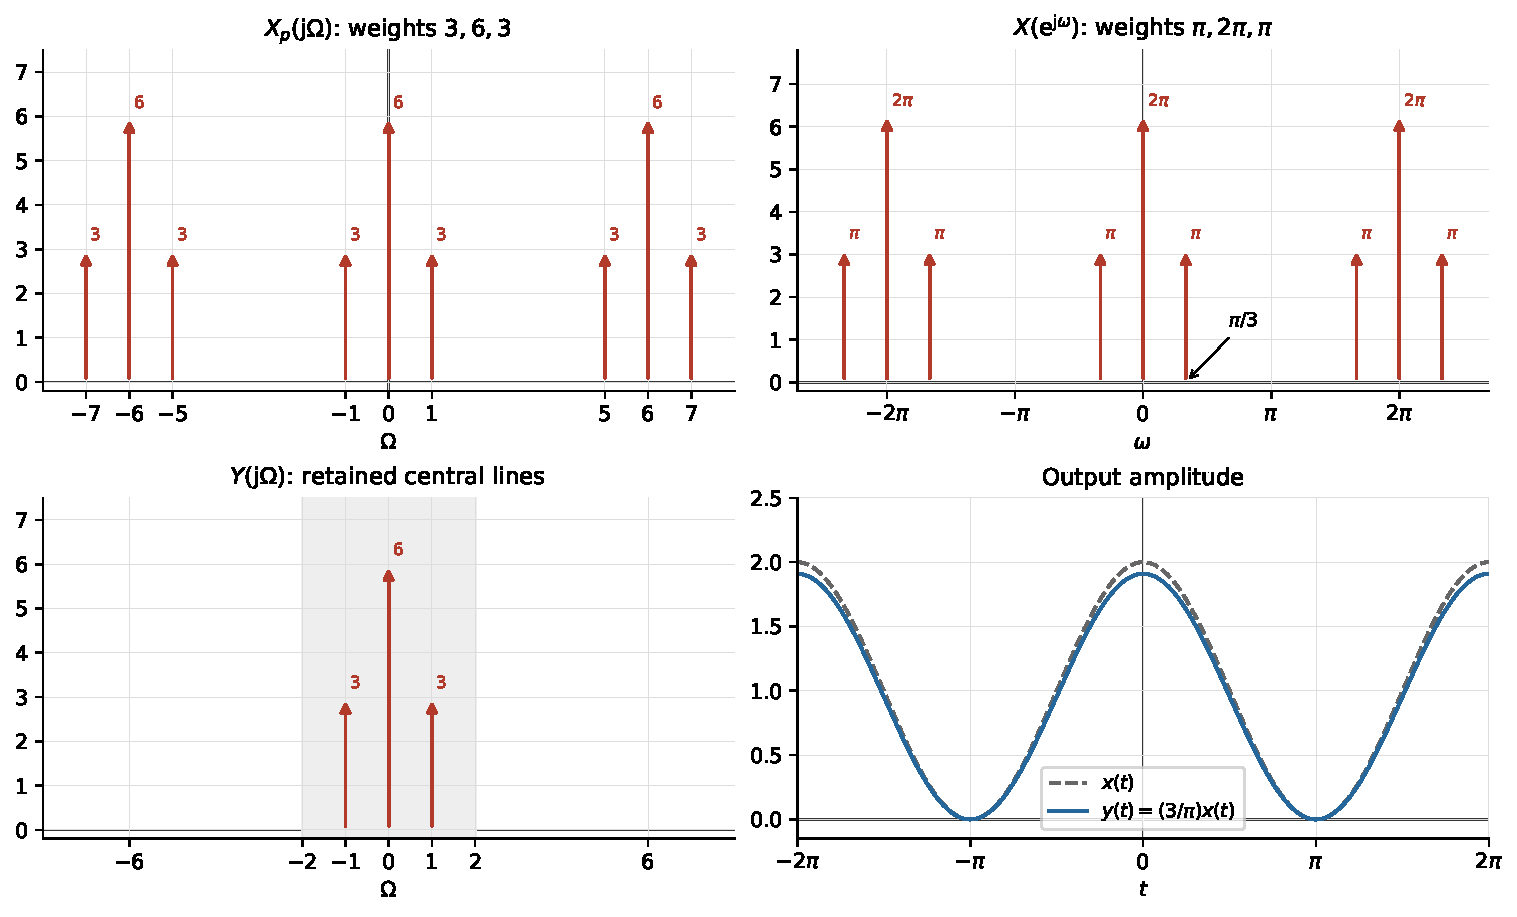
\includegraphics[width=0.95\textwidth]{08-sampling/lines-lowpass-answer.pdf}
    \caption{例题 \ref{ex:sampling-lines-lowpass} 的结果。箭头旁标冲激权重；灰色通带只留下中央三条谱线。右下对照输入与输出，输出幅度为输入的 $3/\pi$。}
    \label{fig:ex-sampling-lines-lowpass-answer}
  \end{figure}
\end{solution}

\begin{technique}
  \hl{连续线谱先按采样角频率复制}，再乘 $1/T$。转到 DTFT 时，频率位置乘 $T$，冲激权重也乘 $T$。经过低通后先列出留下的谱线及权重，再反演；\red{通带位置决定保留哪些频率}，\red{通带高度决定能否恢复原幅度}。
\end{technique}
\begin{workedexample}[由希尔伯特变换求调幅信号的瞬时参数]
  \label{ex:sampling-envelope}
  设
  \[
    x(t)=(1+\tfrac12\cos t)\cos(8t).
  \]
  求 $\widehat{x}(t)$、瞬时包络、瞬时相位和瞬时角频率，并说明为何这里的移相公式可以取等号。输入见\cref{fig:ex-sampling-envelope-question}。
\end{workedexample}

\begin{figure}[H]
  \centering
  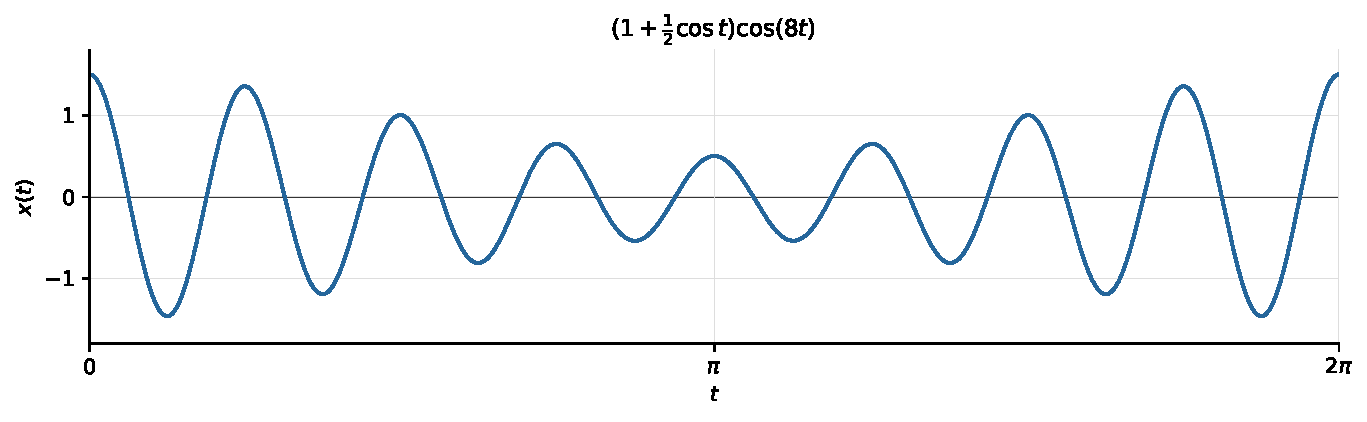
\includegraphics[width=0.9\textwidth]{08-sampling/envelope-question.pdf}
  \caption{例题 \ref{ex:sampling-envelope} 的输入波形 $x(t)=(1+0.5\cos t)\cos(8t)$。}
  \label{fig:ex-sampling-envelope-question}
\end{figure}

\begin{solution}
  先用积化和差将信号分成三条正频率余弦：
  \[
    x(t)=\cos(8t)+\frac14\cos(9t)+\frac14\cos(7t).
  \]
  三个角频率 $7,8,9$ 都为正。分别使用\cref{eq:sampling-hilbert-sinusoid}，
  \[
    \widehat{x}(t)=\sin(8t)+\frac14\sin(9t)+\frac14\sin(7t).
  \]
  用 $\sin(9t)+\sin(7t)=2\sin(8t)\cos t$ 将后两项重新合并，便有
  \[
    \widehat{x}(t)=(1+\tfrac12\cos t)\sin(8t).
  \]
  这也是频带分离条件的直接应用：包络的频率只有 $0,\pm1$，均低于载波 $8$，左右副本不会跨过零频。\red{计算没有使用慢变近似}。

  合成解析信号：
  \begin{align*}
    z(t)&=x(t)+\iu\widehat{x}(t)\\
        &=(1+\tfrac12\cos t)[\cos(8t)+\iu\sin(8t)]\\
        &=(1+\tfrac12\cos t)\e^{\iu8t}.
  \end{align*}
  因为 $1+\frac12\cos t\ge1/2>0$，包络没有零点，也没有负幅度引起的相位翻转。于是
  \[
    A(t)=1+\tfrac12\cos t,\qquad
    \varphi(t)=8t,\qquad
    \Omega_{\mathrm{inst}}(t)=8\ \mathrm{rad/s}.
  \]
  相位写的是展开后的连续分支，可加任意常数 $2\pi k$。幅度随时间变化，但\red{瞬时角频率保持不变}。

  也可核对解析信号的谱线：
  \[
    z(t)=\e^{\iu8t}+\frac14\e^{\iu9t}+\frac14\e^{\iu7t},
  \]
  所以 $Z(\iu\Omega)$ 在 $7,8,9$ 的权重依次为 $\pi/2,2\pi,\pi/2$，负频率全为零，见\cref{fig:ex-sampling-envelope-answer}。

\begin{figure}[H]
  \centering
  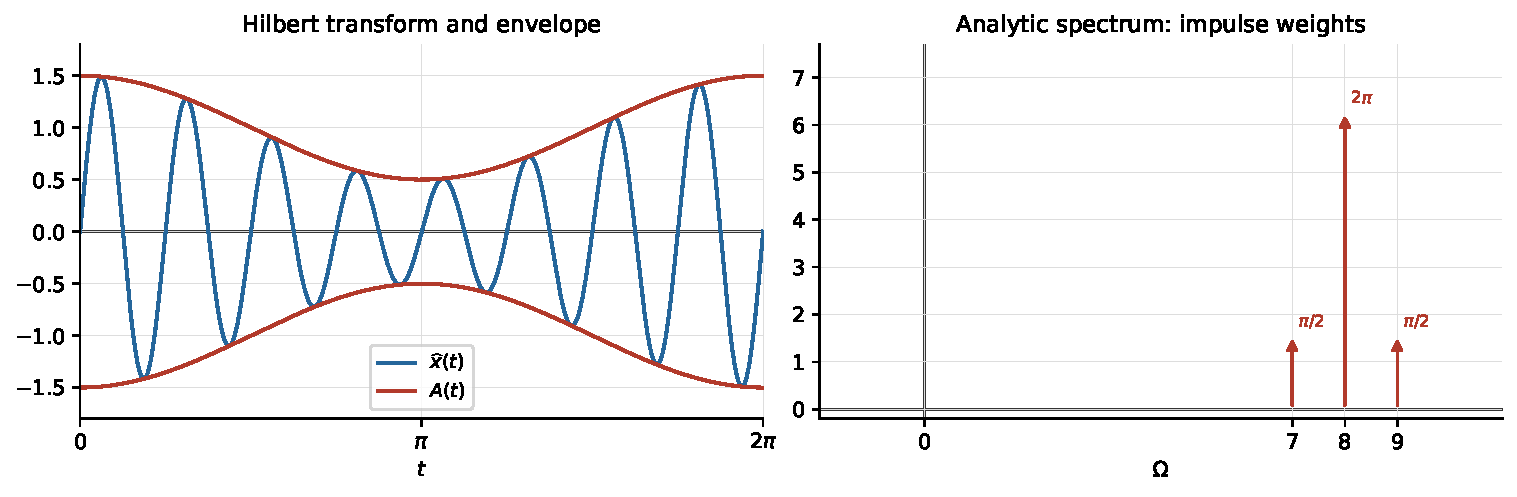
\includegraphics[width=0.9\textwidth]{08-sampling/envelope-answer.pdf}
  \caption{例题 \ref{ex:sampling-envelope} 的希尔伯特变换、包络及解析信号谱线；箭头标权重。}
  \label{fig:ex-sampling-envelope-answer}
\end{figure}
\end{solution}

\begin{technique}
  少数正弦分量构成的调幅信号，\hl{先积化和差，再逐项移相}，\hl{最后合并回包络形式}。\blue{求瞬时相位前检查包络是否恒正}，\blue{求频率前展开相位}。频带跨过零频时，应按每个分量的实际频率符号计算，不能整段套用“余弦变正弦”。
\end{technique}
\endgroup
